\documentclass{article}
\usepackage[utf8]{inputenc}
\usepackage{graphicx}
\usepackage[margin=1in]{geometry}
\usepackage[dvipsnames]{xcolor}
\usepackage{url}
\usepackage{hyperref}
\usepackage[numbers]{natbib} % for numeric references

\begin{document}

\begin{titlepage}
    \begin{center}
        \includegraphics[width=3cm]{figures/MSP-logo.jpg} 
        \vspace{1cm}
        
        \textbf{\LARGE Flipper length and mass in Palmer penguins}\\
        \textbf{\LARGE Correlation comparison between three species: Adelie, Chinstrap, and Gentoo}
        
        \vspace{1.5cm}
        
        \textbf{\Large Polina Shumilina Mironova (ID 6416138)}
        
        \vfill
        
        \large Date: \today
        
    \end{center}
\end{titlepage}

\newpage

\section*{Introduction}
Penguins are one of the main birds found in Antarctica. This project investigates the correlation between their mass and the length of their flippers, as well as whether this correlation varied between the three species found in the Palmer Archipelago: Adelie, Chinstrap, and Gentoo penguins. The research question is \textbf{“How does the correlation between flipper length and body mass differ between the three species of penguins in the Palmer Archipelago?”}. A positive correlation is expected, but it might differ between species due to their morphological differences.

\section*{Data sample}
The dataset contains measurements from 344 penguins. However, after checking for missing values, two penguins were removed from the analysis. The cleaned dataset contained 151 Adelie penguins, 68 Chinstrap penguins, and 123 Gentoo penguins. The variables used in this analysis were species, flipper length in millimetres, and body mass in grams. 
The dataset was obtained from Kaggle~\cite{penguin_dataset}.

\section*{Results and discussion}
The data was analysed in Python using pandas and matplotlib libraries. Pearson's correlation coefficient, $r$, was calculated between flipper length and body mass for all penguins together and then separately for each species. Mean body mass and mean flipper length were also calculated, together with the standard error of the mean.
For all 342 penguins, flipper length and body mass showed a strong positive correlation of $r=0.871$.
When the species were analysed separately, the correlations were:
\begin{itemize}
    \item Adelie: $r=0.468$
    \item Chinstrap: $r=0.642$
    \item Gentoo: $r=0.703$
\end{itemize}
Gentoo penguins had the strongest within-species correlation, followed by Chinstrap and Adelie penguins.
The mean body mass was $3700.66 \pm 37.32$ g for Adelie, $3733.09 \pm 46.61$ g for Chinstrap, and $5076.02 \pm 45.46$ g for Gentoo penguins, where the uncertainty is the SEM. Mean flipper lengths were $189.95 \pm 0.53$ mm, $195.82 \pm 0.87$ mm, and $217.19 \pm 0.59$ mm, respectively.
\begin{figure}[h]
    \centering

    \begin{minipage}{0.48\textwidth}
        \centering
        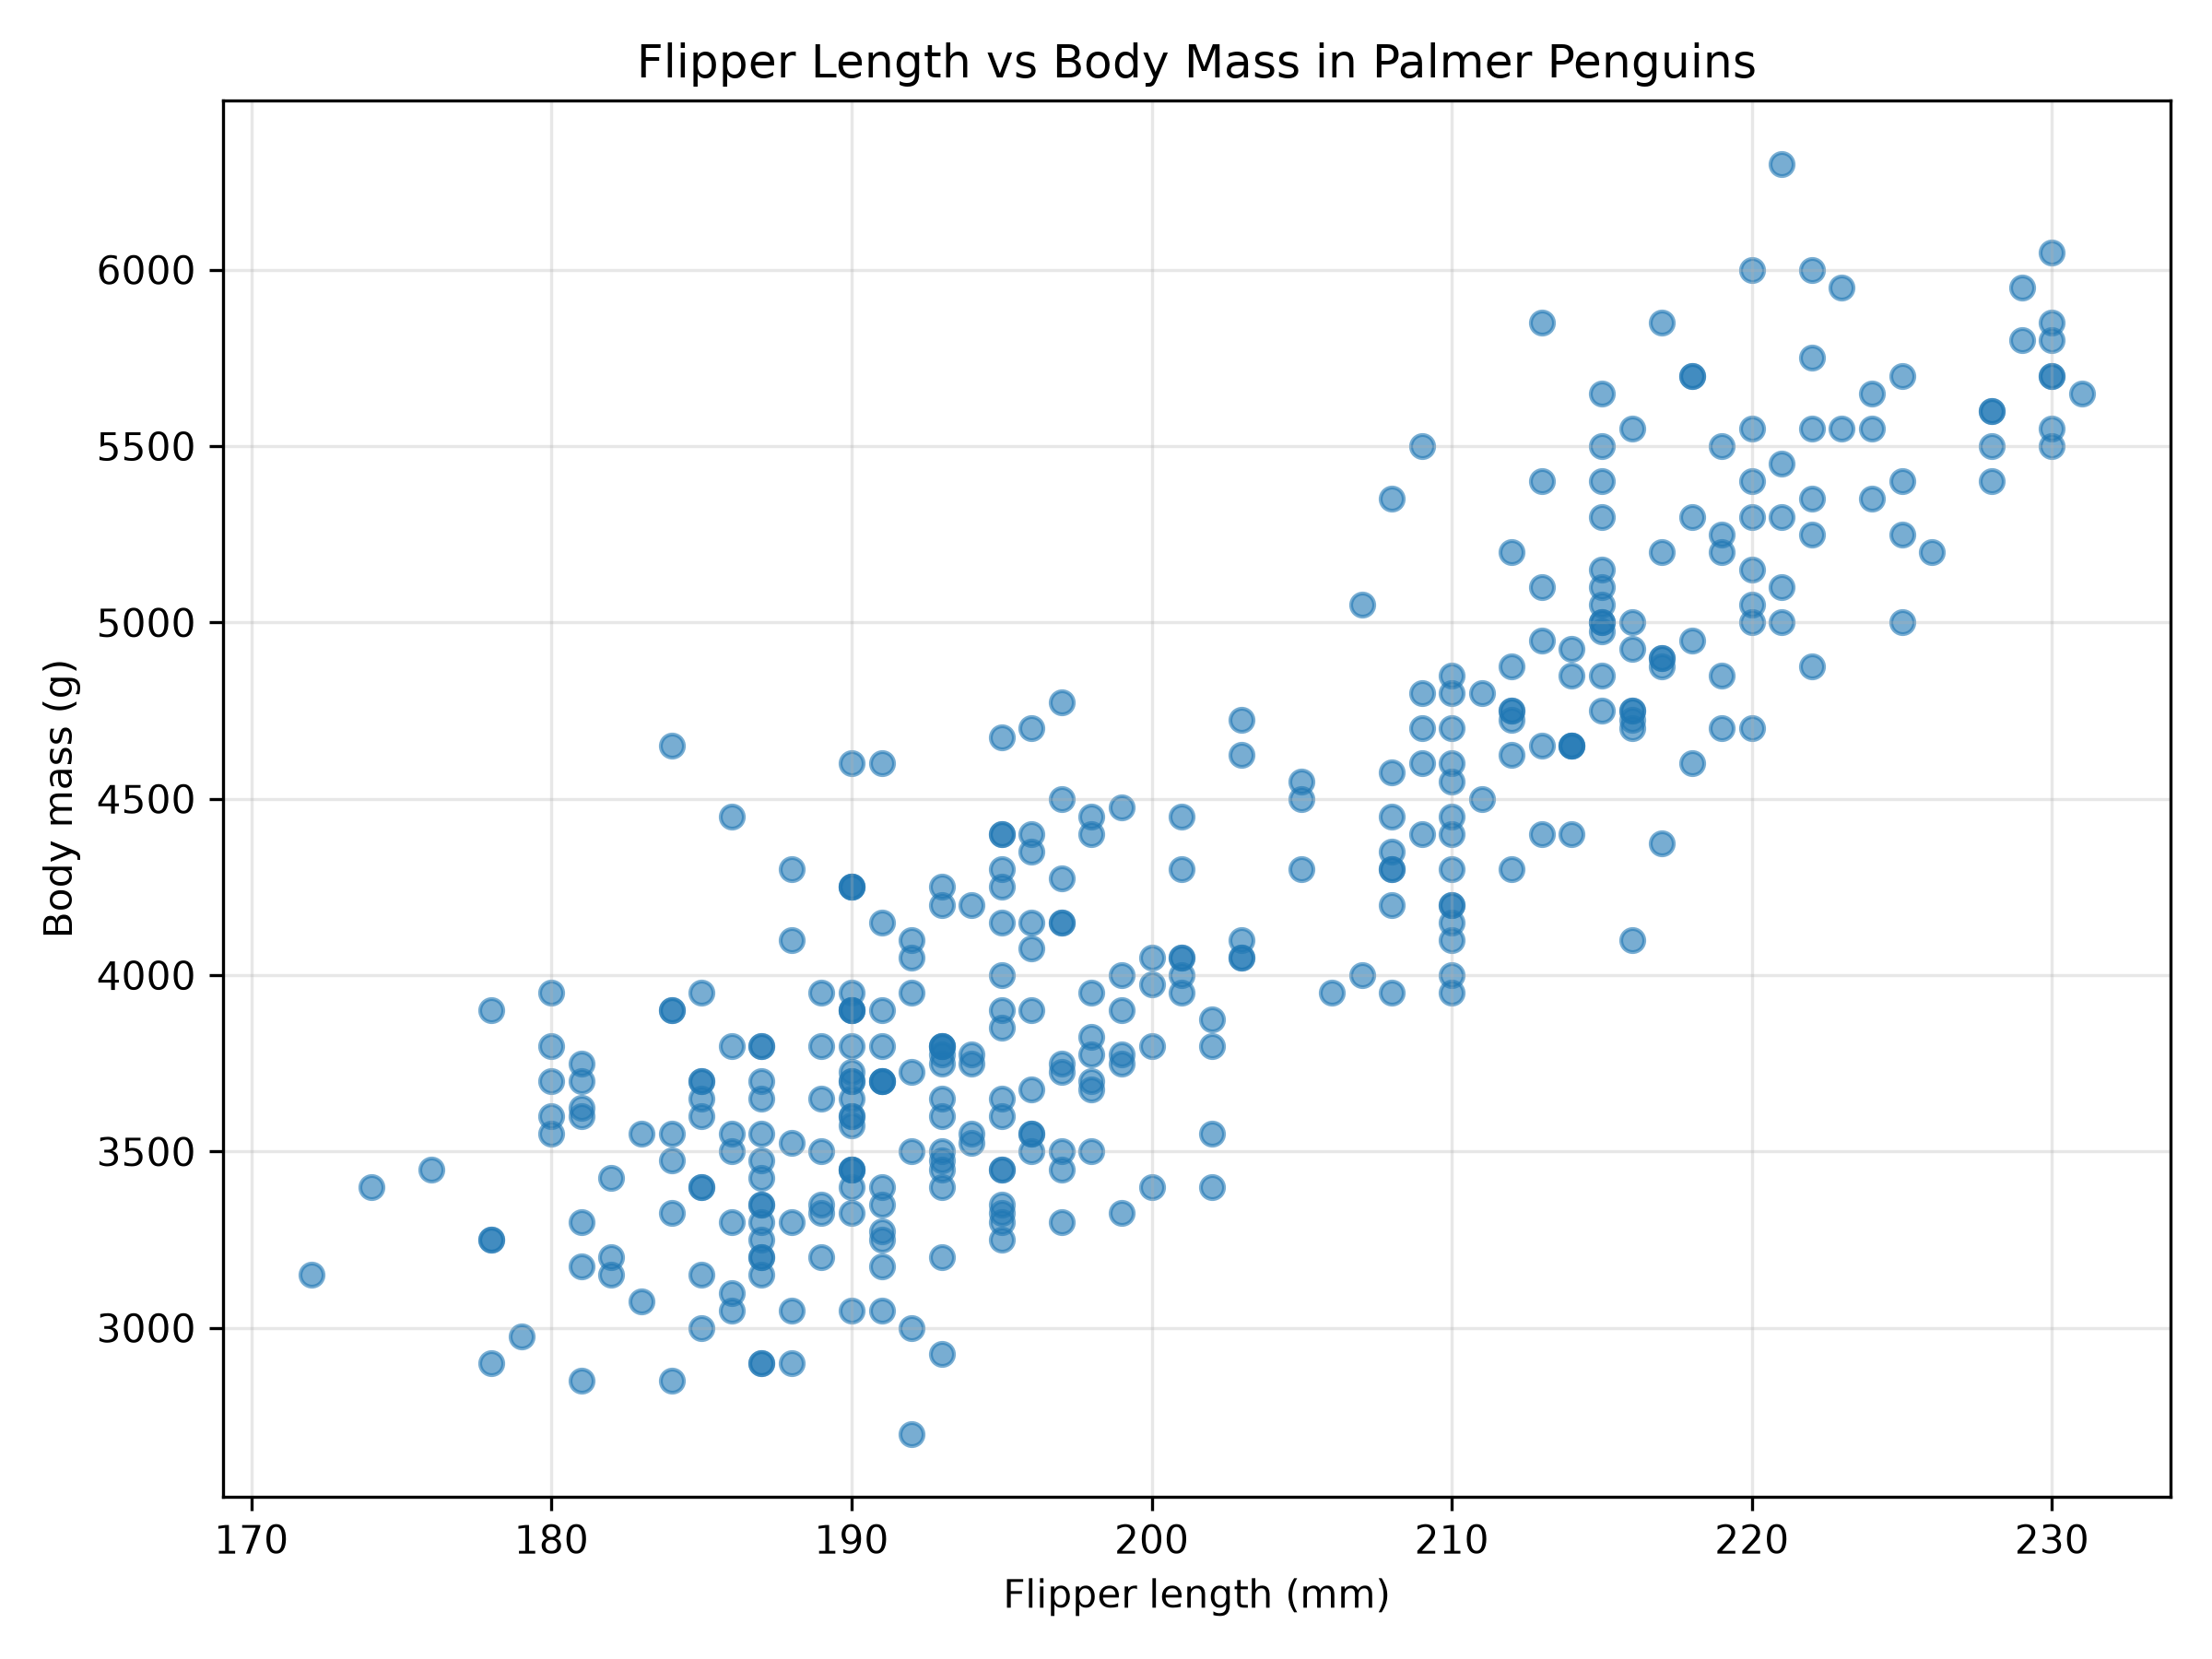
\includegraphics[width=\textwidth]{penguin_scatter.png}
        \textbf{(a)}
    \end{minipage}
    \hfill
    \begin{minipage}{0.48\textwidth}
        \centering
        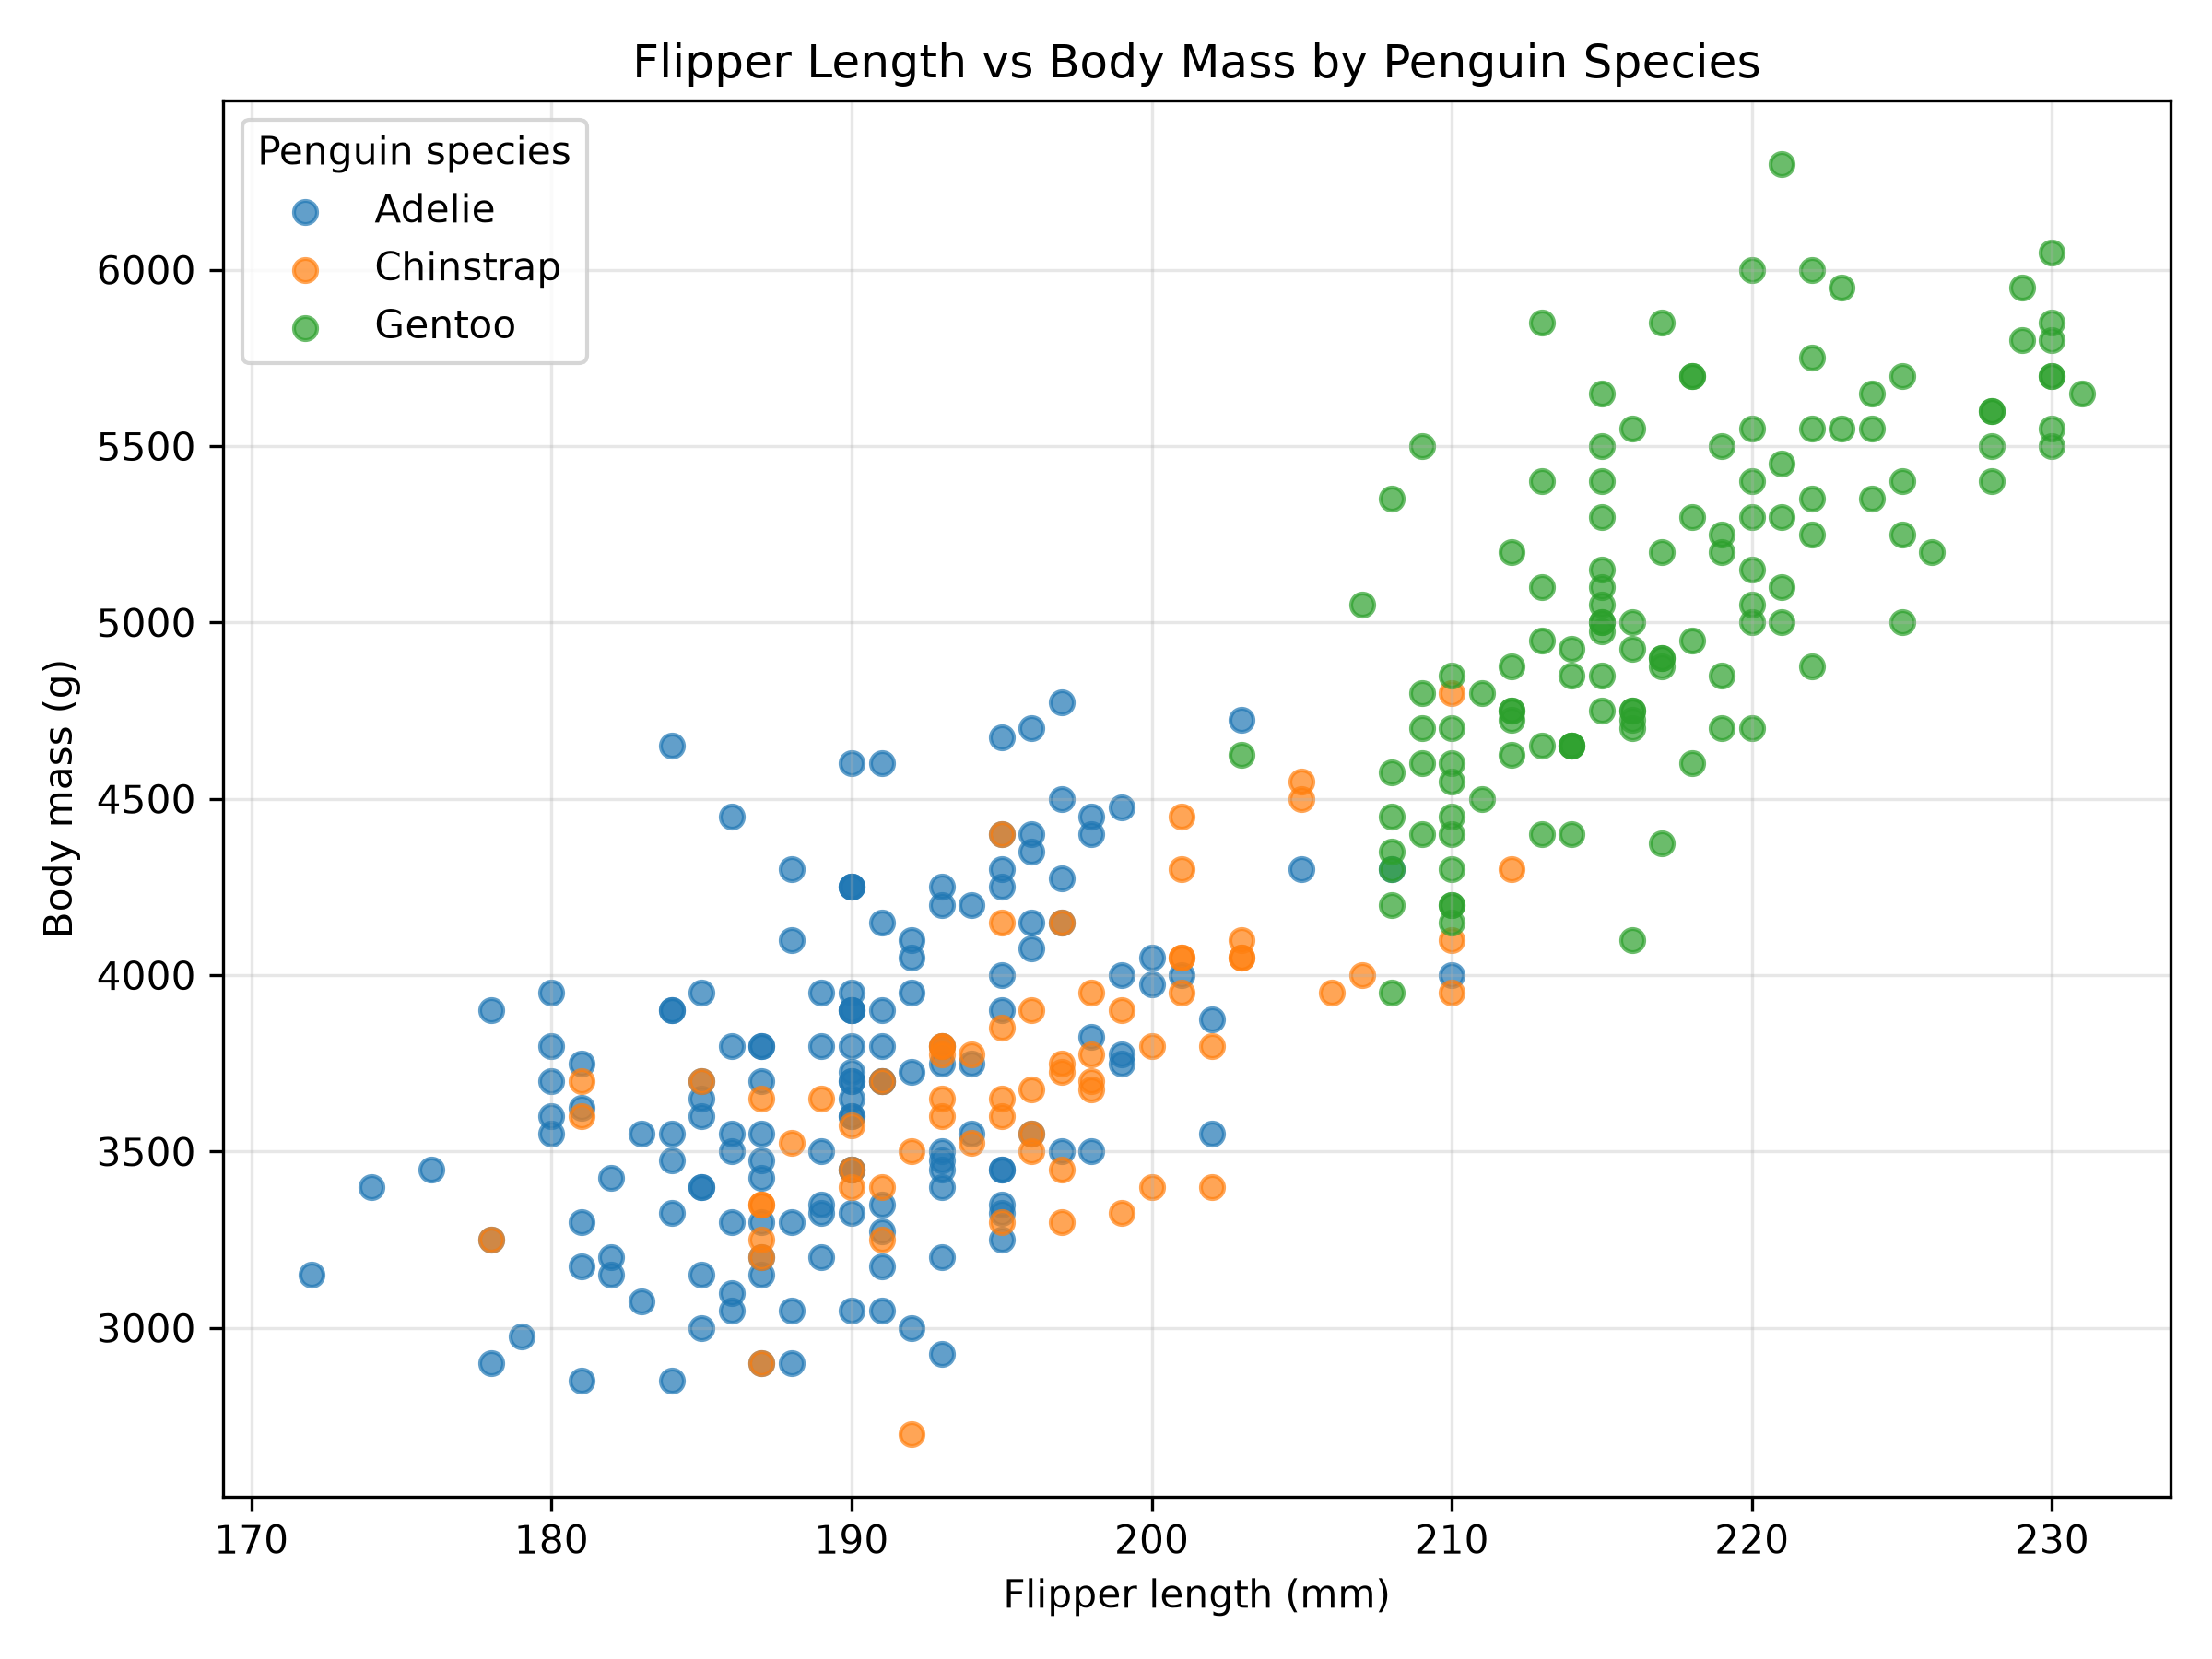
\includegraphics[width=\textwidth]{penguin_species_scatter.png}
        \textbf{(b)}
    \end{minipage}

    \caption{Relationship between flipper length and body mass in Palmer penguins. (a) All 342 penguins analysed together. (b) The same relationship shown separately for Adelie, Chinstrap, and Gentoo penguins.}
    \label{fig:penguin_scatter}
\end{figure}

\section*{Conclusion}
The overall correlation of $r=0.871$ was stronger than the correlation within any individual species. Figure~\ref{fig:penguin_scatter}a shows the strong positive relationship when all penguins are analysed together, while Figure~\ref{fig:penguin_scatter}b shows that the three species form distinct groups. In particular, Gentoo penguins tend to have both greater body mass and longer flippers. These differences between species therefore contribute to the stronger overall correlation. One possible explanation for the positive relationship is that flipper length and body mass are both related to the overall body size of a penguin. Previous research on Adelie, Chinstrap, and Gentoo penguins has also found differences in morphological characteristics and body mass between species and sexes~\cite{gorman2014}. Therefore, species and other biological factors may contribute to the relationship observed in this analysis. However, correlation alone cannot establish that longer flippers cause greater body mass, and other factors such as sex and seasonal variation in body mass may also influence the measurements.

\begin{thebibliography}{9}

\bibitem{penguin_dataset}
P. Pandey,
\textit{Palmer Archipelago (Antarctica) Penguin Data}.
Kaggle.
Available at:
\href{https://www.kaggle.com/datasets/parulpandey/palmer-archipelago-antarctica-penguin-data}
{https://www.kaggle.com/datasets/parulpandey/palmer-archipelago-antarctica-penguin-data}.

\bibitem{gorman2014}
K. B. Gorman, T. D. Williams, and W. R. Fraser,
\textit{Ecological Sexual Dimorphism and Environmental Variability within a Community of Antarctic Penguins (Genus Pygoscelis)}.
PLoS ONE, 9(3), e90081, 2014.


\end{thebibliography}
\end{document}
